% !TeX spellcheck = en_US

\chapter{Overview}

%\todo[inline]{
%Review CS: Chapter One should be a motivation including history of developements, \newline rationale and target reader groups (sntadarization bodies, developers, practitioners, researchers).
%\newline
%AF: See preface\\
%CS: Hochkommas und Bindestriche im pdf nicht alle lesbar, oft mt Umlauten gedruckt!
%}

To facilitate the understanding of the later sections, we will introduce the concept of subject-oriented process modeling with the modeling language Parallel Activity Specification Scheme (PASS). Additionally, we will give a short introduction to ontologies --- especially the Web Ontology Language (OWL) --- and to Abstract State Machines (ASM) as underlying concepts of this standard document.

\section{Subject Orientation and PASS}
\label{SubjectOrient} 

%\index{subject}

%\sidepar{Text in the sidebar}

In this section, we lay the ground for the Parallel Activity Specification Scheme (PASS) as a language for describing processes in a subject-oriented way. It will not a complete description of all PASS features, but it is a first impression and introduction to the principle of subject-orientation. The detailed concepts are defined in later chapters.

\subsubsection{The Term Subject in Subject-Orientation}
%\index{subject}

The term \textit{subject} has manifold meanings, depending on the discipline or domain it is used in. In philosophy, a subject is an observer and an object is a thing observed. In the grammar of many natural languages, the term subject has a slightly different meaning. "According to the traditional view, the [grammatical] subject is the doer of the action (actor) or the element that expresses what the sentence is about (topic)."~\cite{article:GeneralSubject}. In the English the term subject can also be used as a synonym for \textit{topic} as, e.g., the \textit{subject} of an e-mail. 

However, it is the first part of the second meaning that subject-orientation as a paradigm and PASS as a modeling language refer to in their concept. The term \textit{subject} corresponds to the concept of \textit{doer of an action}\footnote{In contrast to e.g. talks to e.g. ontology description languages, like RDF  (see section \ref{IntroOntology}), where term \textit{subject} means the topic what the "sentence" is about}.

\subsection{Subject-driven Business Processes}

In principle, subjects are the active entities in a specific process context that posses a behavior. A specification of a subject does not say anything about the technology used to execute the described behavior. This is different to other approaches, such as multi-agent systems, that usually imply a technical/software solution consisting of executable source code.

Subjects communicate with each other by exchanging information in form of \textit{messages}. Messages have a name and a payload. The name should express the topic or content of a message informally. The payload is the data (business objects) transported. 

During the execution of a (business) process, a subject sends messages to other subjects, expects messages from other subjects, and executes internal actions, such as calculating a price, storing an address, etc.. All these activities are done in sequences as no single processor or human can really multi-task. The possible sequence is defined in a subject's behavior specification. Subject-oriented process specifications are always embedded in a context. A context is defined by the business organization and the technology by which a business process\todo{Add glossary to the document} is executed.

Subject-oriented system development has been inspired by various process algebras (see e.g. \cite{book:S-BPM}, \cite{book:CCS}, \cite{book:Pi-Calculus}, \cite{book:CSP} ), by the basic structure of nearly all natural languages (Subject, Predicate, Object) and the systemic sociology developed by Niklas Luhmann \cite{book:LuhmannLeicht},\cite{book:Luhmann}  and J\"urgen Habermas \cite{book:HabermasLeicht}, \cite{book:Habermas}. In the active voice of many natural languages a complete sentence consists of the basic components subject, predicate and objects. The subject represents the active element, the predicate the action and the object is the entity on which the action is executed. According to the organizational theory developed by Luhmann and Habermas the smallest organization consists of communication executed between at least two information processing entities (Note, this is a definition by a sociologist, not by a computer scientist) \cite{book:Luhmann}. Figure \ref{fig4} summarizes the different inspirations of subject orientation. The enhancements, such as the graphical notation, constitute the subject oriented approach and will be detailed in the following sections.

\begin{figure} [ph!]
	\centering
	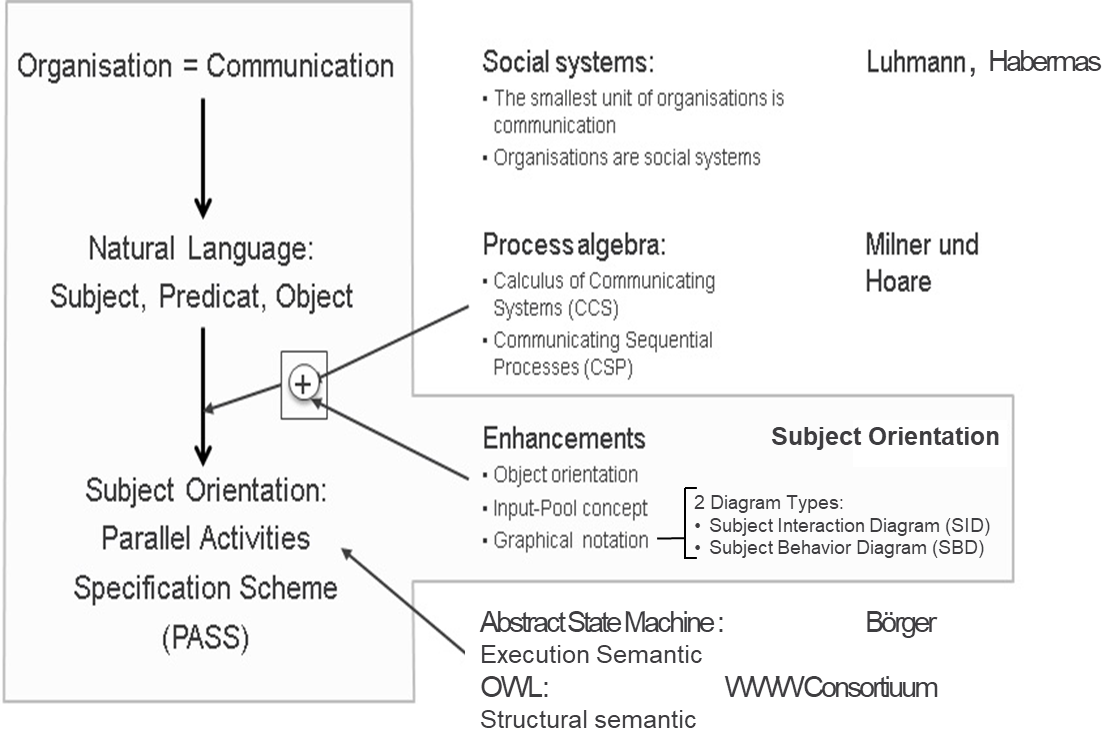
\includegraphics [width=1.0\linewidth]{Figures/fundamentals.png} 
	\caption{Fundamentals of Subject Orientation}
	\label{fig4}
\end{figure}

Particularly we describe how these various ingredients are combined in an orthogonal way to a modeling language for scenarios in which active entities have a certain importance. This language is called Parallel Activity Specification Schema (PASS).\\

\subsection{Subject-Orientation}

Consequently the term Subject-Orientation may be defined as following: 

Subject-Orientation is a modeling or description paradigm for processes that is derived from the structure of natural languages. It requires the explicit and continuous consideration of active entities within the bounds of a process as the conceptual center of description. Active entities (subjects) and passive elements (objects) must always be distinguished and activities or task can only be described in the context of a subject. The interaction between subjects is of particular importance and must explicitly be described as exchange of information that cannot be omitted \cite{elstermann:diss}

\subsection{PASS}

All the previously given concepts have been adapted into a simple graphical notation, that is the \textit{Parallel Activity Specification Schema} - or PASS . Following the principle of subject-orientation,the main concept of PASS is that, first the interaction between Subjects is described and only afterwards the behavior of subjects can be modeled individually. The details are given in the following sections.

\subsection{Modeling Subject Interaction}

We introduce the basic concepts of subject-oriented process modeling with a simple  \textit{order process}. In that process, a customer sends an \textit{order} to the order handling department of a supplier. He is going to receive an order confirmation and the ordered product by the shipment company. Figure \ref{fig:ordercomstructure1} shows the communication structure of that process. There all involved subjects and the exchanged messages can easily be discerned. 

%\strictpagecheck
\begin{figure}[htbp]
	\centering
	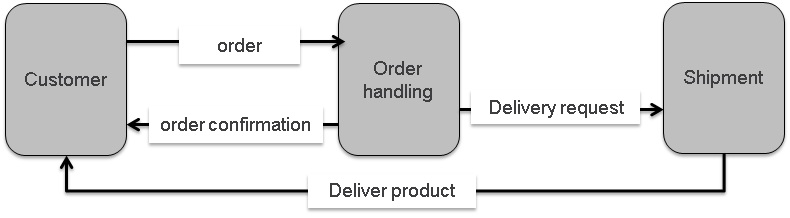
\includegraphics[width=0.7\linewidth]{Figures/Ontology/SubjectExecution/OrderComStructure}
	\caption[The Communication Structure of a simple Order Process]{The Communication Structure of a simple Order Process}
	\label{fig:ordercomstructure1}
\end{figure}

It is assumed that  each subject has a so-called \textit{input pool} which is basically its mailbox for receiving messages. This input pool can be structured via rules according to the requirements in given process context. The modeler can define how many messages of which type and/or from which sender can be deposited and what the reaction is if these restrictions are violated. This means the synchronization through message exchange can be specified for each subject individually.

Messages should have their meaning expressed by their name. A formal semantics is given by their use and the data which are transported with a message. 


\subsection{Modeling Subject Behavior}

Figure \ref{fig:ordercustomerorderhandling} depicts the behavior of the subjects "customer" and "order handling".

%\strictpagecheck
\begin{figure}[htbp]
	\centering
	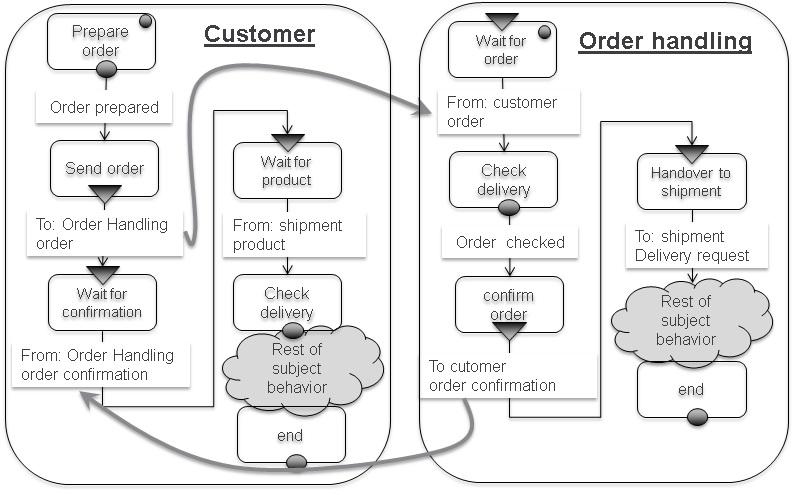
\includegraphics[width=0.9\linewidth]{Figures/Ontology/SubjectExecution/OrderCustomerOrderHandling}
	\caption[The Behaviors of the Subjects from \ref{fig:ordercomstructure1} ]{The Behaviors of the Subjects from \ref{fig:ordercomstructure1}}
	\label{fig:ordercustomerorderhandling}
\end{figure}

In the first state (Do State) of its behavior, the subject "customer" executes the \textit{internal function}  "Prepare order". When this function is finished the transition "order prepared" follows. It basically states the condition that must be fulfilled in order to continue. In the succeeding (Send) state "send order" the message "order" is sent to the subject "order handling". After this message is sent (deposited in the input pool of subject "order handling"), the subject "Customer" is allowed to go into the (Receive) state "wait for confirmation". If this message is not in the input pool the subject stops its execution until the corresponding message arrives in the input pool and the according receive transition condition is fulfilled. On arrival, the subject removes the message from the input pool and follows the transition into state "Wait for product" and so on.

The subject "Order Handling" waits for the message "order" from the subject "customer". If this message is in the input pool it is removed and the succeeding function "check order" is executed and so on.

In summary, the behavior of each subject describes in which order it sends and receives (expects) messages, and performs internal functions. Messages transport data from the sending to the receiving subject and internal functions operate on internal data of a subject. These data aspects of a subject are described in section \ref{SUbjects-Objects}. 

%\subsection{Advanced Subject Behavior Modeling}

%In a dynamic and fast-changing world, processes need to be able to capture known but unpredictable events. In our example let us assume that a customer can change an order. This means the subject "customer" may send the message "Change order" at any time. Figure\todo{AF: Bild und Text passen nicht Change order} \ref{fig:ordercomstructure2} shows the corresponding communication structure, which now contains the message "change order".

%%\strictpagecheck
%\begin{figure}[htbp]
%	\centering
%	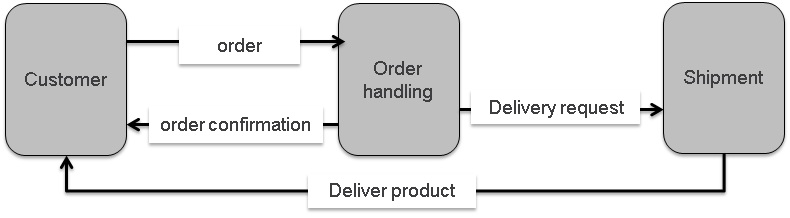
\includegraphics[width=0.7\linewidth]{Figures/Ontology/SubjectExecution/OrderComStructure}
%	\caption[The Communication Structure with Change Message]{The Communication Structure with Change Message}
%	\label{fig:ordercomstructure2}
%\end{figure}

%Due to this unpredictable event, the behavior of the involved subjects needs also to be adapted. Figure \ref{fig:ordercustomerchange} illustrates the respective behavior of the customer. 

%\strictpagecheck
%\begin{figure}[htbp]
%	\centering
%	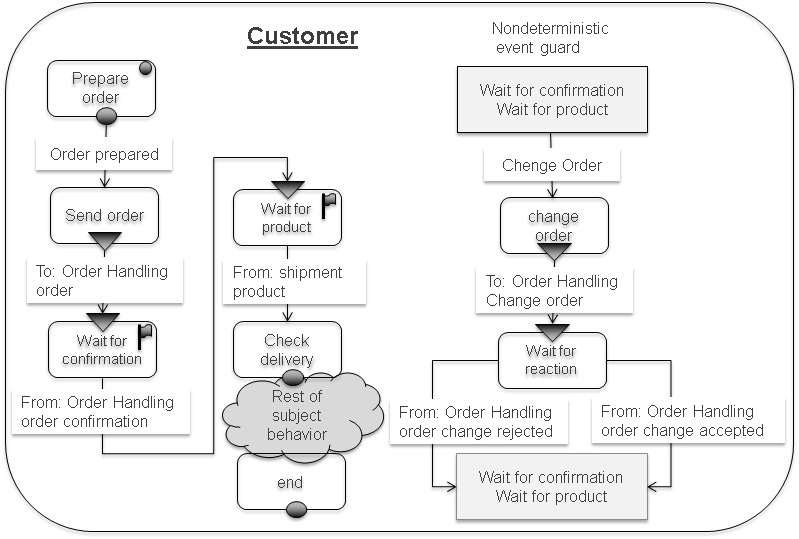
\includegraphics[width=0.9\linewidth]{Figures/Ontology/SubjectExecution/OrderCustomerChange}
%	\caption[Customer is allowed to Change Orders]{Customer is allowed to Change Orders}
%	\label{fig:ordercustomerchange}
%\end{figure}

%The subject "customer" may have the idea to change its order in the state "wait for confirmation" or in the state "wait for product". The flags in these states indicate that there is a so-called behavior extension described by a so-called nondeterministic event guard [12, 22]. The non-deterministic event created in the subject is the idea "change order". If this idea comes up, the current states, either "wait for confirmation" or "wait for product", are left, and the subject "customer" jumps into state "change order" in the guard behavior. In this state, the message "change order" is sent and the subject waits in the state "wait for reaction". In this state, the answer can either be "order change accepted" or "order change rejected". Independently of the received message the subject "customer" moves to the state "wait for product". The message "order change accepted" is considered as confirmation, if a confirmation has not arrived yet (state "wait for confirmation"). If the change is rejected the customer has to wait for the product(s) he/she has ordered originally. Similar to the behavior of the subject "customer" the behavior of the subject "order handling" has to be adapted.

\subsection{Subjects and Data}
\label{SUbjects-Objects}

Up to now, we did not explicitly mention data or rather the concept of data, even though they are necessary to get complete sentences comprising subject, predicate (verbs), and object. In subject-orientation (data-)objects have their place\footnote{Theoretically, the means subject-oriented modeling and object-oriented modeling are 100\% compatible In regards to natural languages it must be understood that pure object-oriented means are akin the passive sentence structures where the subject may be omitted, while subject-oriented descriptions follow the structure of active sentences, that are much easier to understand. }


It is assumed that each subject posses an individual "database" to allow to store objects of arbitrary complexity. Similarly, messages may have a data \textit{payload} representing the transport of data between subjects.
Figure \ref{fig:subjectobject} displays how subjects and objects are connected in the classical way. The internal function  "prepare order" uses or manipulates internal data to prepare the data for the order message. This order data object is sent as the \textit{payload} of the message "order".

%\strictpagecheck
\begin{figure}[htbp]
	\centering
	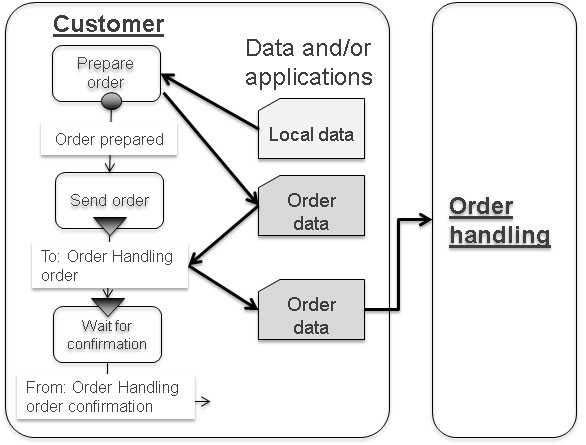
\includegraphics[width=0.9\linewidth]{Figures/Ontology/SubjectExecution/SUbjectObject}
	\caption[Subjects and (Data-)Objects]{Subjects and (Data-)Objects}
	\label{fig:subjectobject}
\end{figure}


Modeling wise, internal functions in a subject can be described as the (passive) methods of a specific data-object or as function calls implemented in a service, if a service-oriented architecture is available.

The functions of send and receive states are assumed to always have an additional method that transfer data between messages and internal data store of a subject. If a message is sent, the method writes data values into to the sent message, and if a message is received the corresponding method is used to copy the received data into the subject's data store. In other words, subject either use synchronous services as an implementation of functions, or asynchronous services that are implemented through other subjects or even through complex processes consisting of multiple subjects themselves. Consequently, the concept Service Oriented Architecture (SOA) is complementary to S-BPM: Subjects are the entities which use the services offered by SOAs.

\section{Introduction to Ontologies and OWL }
\label{IntroOntology}

This short introduction to ontology, the Resource Description Framework (RDF), and the Web Ontology Language (OWL) will help to get an understanding of their usage as definition technologies for Subject-Oriented Modeling and Implementation standard in the form of the PASS ontology that is outlined in sections \ref{PASSStruct} and \ref{PASSExec}.

Ontologies are a formal collections of knowledge or descriptions about the world. They are being used to structure the knowledge of  various domains using taxonomies and classification networks. They often use structures similar to human languages, where nouns in statement-sentences represent objects or classes of objects and the verbs represents relations between the objects of classes. (e.g. \textit{"PASS" "is-a" "process modeling language"})

In computer- and information science, an ontology is a collection or representation of formal names, class definitions, properties, relations between them, and according entities with their relations  - usually in regards to a specific thematic domain.


\subsection{RDF and OWL}

The Resource Description Framework (RDF)\cite{rdf:rdf} provides a graph-based data model or framework for structuring data as statements about resources. A "resource" may be any "thing" that exists in the world: a person, place, event, book, museum object, but also an abstract concept like data objects. Figure \ref{fig:classes-properties}  shows an RDF graph.

%\strictpagecheck
\begin{figure}[h]
	\centering
	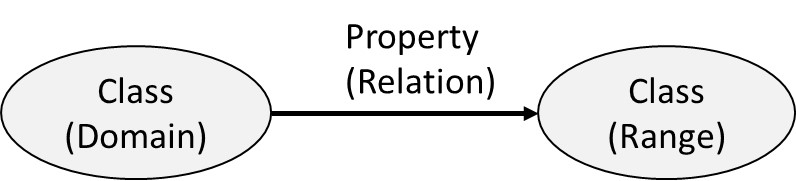
\includegraphics[width=0.6\linewidth]{Figures/Ontology/Introduction/Classes-Properties}
	\caption[RDF graphic]{RDF graphic}
	\label{fig:classes-properties}
\end{figure}

RDF is based on the idea of making statements about resources (in particular web resources) in expressions of the form subject–predicate–object, known as triples. The subject denotes the resource, and the predicate denotes traits or aspects of the resource and expresses a relationship between the subject and the object. In the context of ontology, the term subject expresses what the sentence is about (topic), it must not be confused with term subject in the context of Subject-Orientation (see \ref{SubjectOrient}).

For describing ontologies several formal languages have been developed. One widely used language is OWL (Web Ontology Language)\cite{w3c:owl}, which is based on, or a kind of extension to the Resource Description Framework (RDF).

OWL introduces and allows to use the modeling mechanisms of classes, properties, and instances. Classes represent terms also called concepts. Classes have properties and instances are individuals of one or more class.

A class is a type of thing. A type of "resource" in the RDF sense can be a person, place, object, concept, event, etc.. Classes and subclasses form a hierarchical taxonomy and members of a subclass inherit the characteristics of their parent class (superclass). Everything true for the parent class is also true for the subclass. A member of a subclass "is a", or "is a kind of" its parent class.

OWL Ontologies define a set of properties used in a specific knowledge domain. In an ontology context, properties relate members of one class to members of another class or a literal.

Domains and ranges define restrictions on properties. A domain restricts what kinds of resources or members of a class can be the subject of a given property in an RDF triple. A range restricts what kinds of resources/members of a class or data types (literals) can be the object of a given property in an RDF triple.

Entities belonging to a certain class are instances of this class or individuals. A simple ontology with various classes, properties and individual is shown below:

\subsubsection{Ontology statement examples:}

\begin{itemize}
	\item \textbf {Class definition statements:}
	\begin{itemize}
		\item Parent \texttt{isA} Class
		\item Mother \texttt{isA} Class
		\item Mother \texttt{subClassOf} Parent
		\item Child \texttt{isA} Class
	\end{itemize}
	\item \textbf {Property definition statement:}
	\begin{itemize}
		\item \texttt{isMotherOf} is a relation between the classes Mother and Child
	\end{itemize}
	\item \textbf{Individual/instance statements:}
	\begin{itemize}
		\item MariaSchmidt \texttt{isA} Mother
		\item MaxSchmidt \texttt{isA} Child
		\item MariaSchmidt \texttt{isMotherOf} MaxSchmidt
	\end{itemize}
\end{itemize}

\section{Introduction to Abstract State Machines}

Where the OWL/RDF ontology concepts will be used to define the static structure of subject-oriented process models. The execution semantics will be specified using the concept of \textit{Abstract State Machines}. This section will give a short introduction into this topic in order to help the understanding of their usage in section \ref{PASSExec}.

An abstract state machine (ASM) is a state machine\footnote{State Machines and therefore also abstract state machines are both formal description concepts in theoretical computer science used to describe or define the execution order of a system - e.g. a software program} operating on states that are arbitrary data structures (structure in the sense of mathematical logic, that is a nonempty set together with several functions (operations) and relations over the set). In simpler terms, where in standard state machines the states are explicitly defined (e.g. \textit{state01}, \textit{state02}), in an ASM the states or only implicitly or abstractly defined (e.g. \textit{"a state where a data value is x"}).

The language of the so-called Abstract State Machine uses only elementary If-Then-Else-rules which are typical also for rule systems formulated in natural languages, i.e., rules of the (symbolic) form:

\medskip
$\boldsymbol{if} \textit{Condition} \boldsymbol{then} \textit{ACTION}$
\medskip

with arbitrary \textit{Condition} and \textit{ACTION}. The latter is usually a finite set of assignments of the form \textit{f (t1, ..., tn) := t}. The meaning of such a rule is to be performed in any given state, when the indicated condition holds true - the \textit{CONDITION} there indirectly defines that state.

The unrestricted generality of the used notion of \textit{CONDITION} and \textit{ACTION} is guaranteed by using so-called Tarski structures as ASM-states, i.e., arbitrary sets of arbitrary elements with arbitrary functions and relations defined on them. These structures are not necessarily fixed, but are themselves updatable by rules of the form above. 

%In the case of business processes, the elements of \textit{CONDITION} and \textit{ACTION}-rules are placeholders for values of arbitrary type and the operations are typically the creation, duplication, deletion, or manipulation (value change) of objects. The so-called views are conceptually nothing else than projections (read: substructures) of such Tarski structures.

An (asynchronous or distributed) ASM consists of a set of agents, each equipped with an individual set of rules in the above given form, called its program. In principle, every agent can evaluated and , if applicable, execute all its rules at any time in one step (in any arbitrary state). In contrast, an ASM, that has only one agent, is called sequential ASM. In general, each agent has its own "time" to execute a step, and a step is independent of the steps of other agents. However there in special cases, multiple agents can also execute their steps in a synchronous manner.

Without further explanations, we adopt usual notations, abbreviations, etc., for example:

% for the typesetting of ASM code some work is required!!
%\lstdefinelanguage{ASM}{C}
%\lstset{language=ASM}
\medskip
$ \mathbf{if} ~ Cond  ~ \mathbf{then} ~ M1 ~ \mathbf{else} ~ M2$
\medskip

instead of the equivalent ASM with two rules:

\medskip
$ \mathbf{if} ~ Cond  ~ \mathbf{then}  M1$
$ \mathbf{if ~ not} ~ Cond  ~ \mathbf{then} ~ M2$
\medskip

Another notation used below is

\medskip
$ \mathbf{let} ~ x ~ = ~ t ~ \mathbf{in} ~ M$
\medskip

for $M(x/a)$, where $a$ denotes the value of $t$ in the given state and $M(x/a)$ is obtained from $M$ by substitution of each (free) occurrence of $x$ in $M$ by $a$.

For details of a mathematical definition of the semantics of ASMs which justifies their intuitive (rule-based or pseudo-code) understanding, we refer the reader to the AsmBook Börger, E., Stärk R. Abstract State Machines. A Method for High-Level System Design and Analysis. Springer, 2003 \cite{book:ASM-2003}.





